\documentclass[dvipsnames]{article}
\usepackage{hyperref}
\usepackage[utf8]{inputenc}
\usepackage[usenames,dvipsnames,svgnames,table]{xcolor}
\usepackage{color}
\usepackage{alltt}
\usepackage{amsmath}
\usepackage{amssymb}
\usepackage{listings}
\usepackage{xcolor}
\usepackage{multicol}
\usepackage{graphicx}
\usepackage{tikz}
\usepackage{multicol}

\setlength{\textwidth}{6.5in}
\setlength{\textheight}{8.9in}
\setlength{\voffset}{-1in}
\setlength{\oddsidemargin}{0in}
\setlength{\evensidemargin}{0in}

\newcommand{\Lim}[1]{\raisebox{0.5ex}{\scalebox{0.8}{$\displaystyle \lim_{#1}\;$}}}

\begin{document}

\noindent Criptografia (2018/2019)
\hfill DCC/FCUP

\begin{center}\LARGE\bf 
  Implementação de Gerador de Chaves RSA em Python \\
\end{center}

\vskip 0.4cm
\hrule
\vskip 0.4cm

\begin{multicols}{2}
  \section{Introdução}
  Pretende-se neste relatório descrever a Implementação de uma função em python, \texttt{genRSAkey(l)} que receba como argumento um tamanho de chave $\ell$ e retorne um tuplo da forma $(n,p,q,e,d)$, respeitando as condições descritas a seguir:
  \begin{itemize}
    \item $n=pq$ sendo $p$ e $q$ primos e por forma a que $log_2(n) \geq \ell$ (ou seja que $n$ tenha na sua representação binária pelo menos $\ell$ bits);
    \item $e$ inteiro coprimo com $(p-1)(q-1)$, ou seja, o máximo divisor comum entre $e$ e $(p-1)(q-1)$ seja 1;
    \item $d$, por forma a que $ed \equiv 1 (mod (p-1)(q-1))$
  \end{itemize}
  
  \section{Geração de primos $p$ e $q$}
  Usando o módulo \texttt{random} do Python, a função \texttt{genRand(l)} gera números ímpares no intervalo $2^{w-1} + 1$ e $2^{w} - 1$ em que $w=\lfloor \frac{\ell}{2} \rfloor$, sendo que todos os números passíveis de serem gerados por \texttt{random.randrange} no intervalo descrito acima são depois \textbf{OR}-ed com $1$ no seu bit menos significativo, aumentando assim a eficiência do gerador, visto que qualquer primo $>2$ é necessariamente ímpar.
  
  \vskip 0.4cm
  
  \subsection{Crivo de Eratóstenes}
  
  Depois de gerado o número $p$ (candidato a primo), verificar-se-á, numa primeira fase, contra um crivo de Eratóstenes, gerado apenas uma vez aquando da chamada de \texttt{genRSAkey(l)} e guardado em \texttt{small\_primes}, contendo os $1000$ primeiros números primos. Se algum destes é factor de $p$, então sabemos que $p$ não é primo, sendo assim necessário invocar \texttt{genRand(l)} novamente e repetir o teste.
  
  \subsection{Teste de Miller-Rabin}
  
  No caso em que o número $p$ gerado passa pelo processo de \textit{sieving} supra descrito sem serem encontrados factores primos, prosseguimos para o teste de primalidade de Miller-Rabin (probabilístico). É de salientar que este último domina a complexidade temporal de \texttt{genRSAkey(l)}. Usar \textit{sieving} é eficaz em minimizar o número de vezes em que é gerado um número composto $p$ e este tem que ser sujeito ao teste de Miller-Rabin, ou seja: se $p$ tem factores primos relativamente pequenos, detectamos desde logo que este é composto, gerando assim um novo $p$ cuja primalidade volta a ser testada pelo mesmo processo. Formalmente, dada uma constante $B$, só serão sujeitos ao teste de M-R os candidatos a primos que se não se revelem $B$\textit{-smooth} \cite{DBLP:journals/dcc/Lenstra00} e neste caso $B$ é o último elemento do crivo de Eratóstenes.
  
  \vskip 0.4cm
  
  \noindent O valor de \texttt{max\_rounds} em \texttt{genRSAkey(l)}, corresponde ao número máximo de testemunhas aleatórias $a$ geradas no intervalo $[2,n-2]$ com relação à primalidade de um inteiro $n$, tal que $n>2$. Já que o teste de M-R retorna \texttt{False} quando $n$ é composto, porque foi gerado um $a$ que é testemunha da existência de factores primos de $n$, então podemos dizer que se $n$ é um número composto, quanto mais iterações do teste de M-R forem feitas para esse $n$, maior é a probabilidade de encontrar uma testemunha a (gerada aleatóriamente) que respeite esses critérios e determine que $n$ não é primo.
  
  \vskip 0.4cm
  
  \noindent Baseando-nos no parágrafo anterior, podemos concluir que: se $n$ é um número composto e ao fim de \texttt{max\_rounds} o teste M-R não retornou \texttt{False}, então $n$ é um "falso primo".\\
  
  \noindent Sejam as variáveis aleatórias:
  
  \begin{itemize}
    \item $Y_k \leftarrow n$ é declarado primo depois de $k$ iterações do teste de M-R;
    \item $X \leftarrow n$ é um número composto (sendo $\overline{X} \leftarrow n$ é um número primo).
  \end{itemize}
  
  % Consultar: https://en.wikipedia.org/wiki/Miller–Rabin_primality_test
  
  \noindent Por \cite{DBLP:journals/dcc/Lenstra00} é possivel mostrar que pelo menos $\frac{3}{4}$ das testemunhas aleatórias em $a \in [2,n-2]$ podem garantir que $n$ é composto, que é o mesmo que dizer que no máximo $\frac{1}{4}$ das testemunhas aleatórias no mesmo intervalo não garantem tal. Com isto podemos dizer que $Pr[Y_k|X] \leq \frac{1}{4}$ para uma iteração do teste de M-R, ou seja $k=1$. Sendo que para todas as $k$ iterações do teste de M-R, é independente a escolha de $a$, mostrou-se em \cite{1204.1657v2} que a probabilidade de erro deste teste pode ser descrita em função de $k$ como $Pr[X|Y_k] \leq (\frac{1}{4})^k$ e que $Pr[Y_k|X]$ é relacionável com $Pr[X|Y_k]$, advindo do teorema de Bayes e conforme detalhado em \cite{1709.09963}.
  
  \vskip 0.4cm
  
  \noindent Em vista dos resultados obtidos escolheu-se um $k=100$, coincidente com \texttt{max\_rounds} na função de geração de tuplos para as chaves RSA, o que admite uma probabilidade de erro igual ou inferior a $\frac{1}{4^{100}}$, algo admissível na geração dos factores primos de $n$ (RSA \textit{modulus}). Para suportar o argumento acima, de acordo com \cite{FIPS} (página 70) é dito que para uma probabilidade de erro até $2^{-112}$, são recomendadas pelo menos $56$ iterações do teste M-R, quando $p$ e $q$ tiverem na sua representação 2048 bits.
  
  \subsection{Noção de \textit{strong primes} em RSA}
  
  Com base na hipótese de Riemann, o teorema dos números primos \cite{rh} implica que para um grande primo $p$, a sua proximidade com relação ao seu sucessor é, em média, $log(p)$ e $\Lim{p \rightarrow \infty}log(p) = \infty$. Isto significa que para números da ordem de $2048$ bits, temos elevada probabilidade de gerar um par $p$ e $q$ que seja seguro no sentido em que $n$ não seja facilmente factorizável, porque $p$ e $q$ não são suficientemente próximos. Mais concretamente, conforme provado em \cite{DBLP:journals/iacr/ErraG09}, devemos garantir que $|p-q| > 2^{\frac{k}{3}}$ (onde $k$ é o número de bits na representação dos primos $p$ e $q$) para que $n$ não seja passível de ser factorizado em tempo polinomial, pelo método de de factorização de Fermat. A variável \texttt{safe\_dist} na função apresentada é usada para a verificação de que os primos gerados satisfazem as condições supra descritas, tratando também o caso em que $p = q$.
  
  \section{Escolha do expoente público}
  Como expoente público, decidimos escolher, de forma estática, $e$ =  65537, uma vez que este número é usado de forma comum como expoente público no RSA.
  
  \vskip 0.4cm
  
  \noindent A razão para ser tão comum deve-se a ser um número de Fermat (${2^{2^n}}+1$), com $n$ = 4; um número primo suficientemente grande para evitar certos ataques ao RSA e a ter um peso de Hamming baixo (número de bits a 1), o que torna a sua computação extremamente rápida.
  
  \section{Cálculo de $d$}
  Para calcular o $d$, utilizamos uma extensão do algoritmo de Euclides, onde $ax + by = gcd(a,b)$, uma vez que esta permite calcular um inverso modular multiplicativo, de forma muito rápida.
  
  \vskip 0.4cm
  
  \noindent Da expressão $ax + by = gcd(a,b)$ ($=1$, porque, neste caso, $a$ e $b$ são primos), pode conferir-se que $ax \equiv 1 (mod (b))$, e da expressão $ed \equiv 1 (mod (p-1)(q-1))$, pode simplesmente apurar-se que $d = e^{-1} (mod (p-1)(q-1))$, o que permite aplicar o algoritmo, para descobrir o $d$.
  
  \section{Conclusões}
  
  Apesar de neste trabalho lidarmos com números de grande magnitude e isso mitigar de certa forma os riscos associados a ataques ao RSA baseados na factorização de $n$, achámos pertinente tomar certas medidas que descrevemos em cima quando justificável. É seguro afirmar que foi atingido o objectivo de geração de tuplos $(n,p,q,e,d)$ em tempo que podemos considerar útil, sendo que no corpo de \texttt{genRSAkey(l)} existem instruções de controlo, por forma a garantir todas as condições referidas na Secção 1 e assegurar a correcção do algoritmo.\\
  
  \noindent Abaixo inclui-se um histograma de frequências para os tempos de execução, na ordem dos segundos, de \texttt{genRSAkey(l)} de um total de $2000$ iterações, em que valores decimais foram arredondados para o inteiro mais próximo.
  
  \vskip 0.2cm
  
  \noindent \scalebox{.5}{
  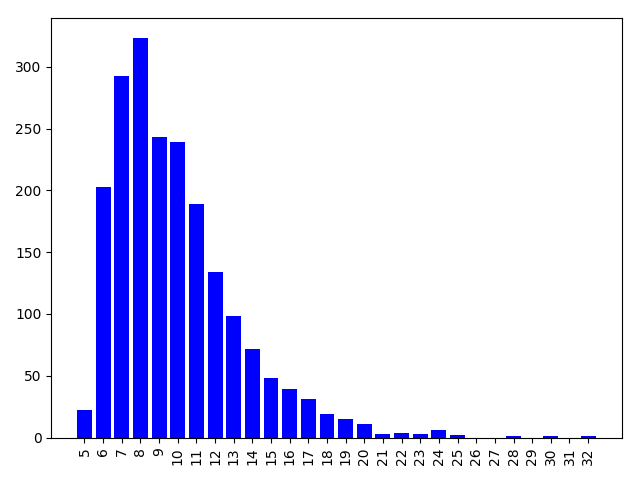
\includegraphics{LPrimeFreqs2000.png}
  }
  
  Da amostra referida de $2000$ tempos de execução, podemos afirmar que o valor esperado do tempo de execução de \texttt{genRSAkey(l)} é aproximadamente $9.94$ segundos.

  \bibliography{report.bib}
  \bibliographystyle{ieeetr}
  
\end{multicols}

\end{document}
